\documentclass[tikz, border=50pt]{standalone}

\usepackage{tikz}
\usepackage{geometry}
\usepackage{medl_colors}
\usepackage{graphicx}

\usetikzlibrary{shapes.multipart, shapes.geometric, arrows.meta}
\usetikzlibrary{matrix,decorations.pathreplacing, calc, positioning,fit}

\graphicspath{ {./images/} }

\begin{document}

\begin{tikzpicture}

\newcommand\cube[7]
{
\draw (#1+#4,#2,#3) -- (#1,#2,#3) -- (#1,#2+#5,#3);
\draw (#1+#4,#2,#3) -- (#1+#4,#2,#3+#6) -- (#1+#4,#2+#5,#3+#6) -- (#1+#4,#2+#5,#3) -- cycle;
\draw (#1+#4,#2+#5,#3) -- (#1,#2+#5,#3) -- (#1,#2+#5,#3+#6) -- (#1+#4,#2+#5,#3+#6);

\coordinate (#7B) at (#1+#4, #2+#5/2, #3+#6/2);
}

%Clustering Blocks
%Input Data
\node (rect) [draw, minimum width=1.5cm,minimum height=3cm] (rect) at (0,0)  {};
\draw[draw, -] ([yshift=-0.1cm]rect.north) -- ([yshift=0.1cm]rect.south) node[midway, anchor=center, fill=white] {$x$}+(0,1mm);
\node[above of=rect, align=center, node distance=2cm] (training) {Input\\Data};

%Cube
\cube{3}{-1.2}{0}{3}{2}{-1.5}{cube1}
\node[align=center] at (4.5,-.2) {Clustering\\Algorithm};

%Model
\node[ellipse, draw=black, minimum width = 4cm, minimum height = 2.5cm,  align=center] (model) at (10.5,3) {Model\\(Clustering\\Rule)};

%Clustered Data
\node[rectangle split, rectangle split parts=7, rectangle split draw splits=false, minimum height=8cm, draw] (rect1) at (10.5, -3) {
    Cluster 1
    \nodepart{two} Cluster 2
    \nodepart{three} .\\.
    \nodepart{four} .\\.
    \nodepart{five} .\\.
    \nodepart{six} .\\.    
    \nodepart{seven} Cluster k
};
\draw[draw, -] (rect1.text split east) -- (rect1.text split west) node[] {};
\draw[draw, -] (rect1.two split east) -- (rect1.two split west) node[] {};
\draw[draw, -] (rect1.six split east) -- (rect1.six split west) node[] {};
\node[above of=rect1, align=center, node distance=2cm] (cluster) {Clustered\\Data};

%World
\node[scale = .5] (inputpic) at (16,-6) {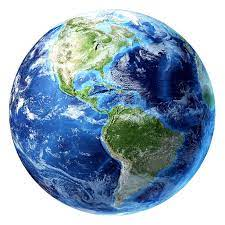
\includegraphics {images/earth.jpeg}};
\node[right of=inputpic, align=center, node distance=2.5cm] {Real\\World};

%Arrows
\draw [-Triangle, draw=green1, line width=1mm] (rect.east) -- ($(rect.east)+(2.2,0)$)  node[] {};
\path (cube1B) edge [-Triangle, out=0,in=180,draw=green1, line width=1mm] node [] {} (model);
\path (cube1B) edge [-Triangle, out=0,in=180,draw=green1, line width=1mm] node [] {} (rect1);
\path (inputpic) edge [Triangle-Triangle, out=90,in=0,draw=green1, line width=1mm] node [] {} (model);
\path (inputpic) edge [Triangle-Triangle, out=175,in=0,draw=green1, line width=1mm] node [] {} (rect1);

%Data Reduction

%Input data
\node (rect) [draw, minimum width=1.5cm,minimum height=3cm] (rect2) at (0,-11)  {};
\draw[draw, -] ([yshift=-0.1cm]rect2.north) -- ([yshift=0.1cm]rect2.south) node[midway, anchor=center, fill=white] {$x$}+(0,1mm);
\node[above of=rect2, align=center, node distance=2cm] (training) {Input\\Data};

%Cube
\cube{3}{-12.2}{0}{3}{2}{-1.5}{cube2}
\node[align=center] at (4.5,-11.2) {Data Reduction\\Algorithm};

%model
\node[ellipse, draw=black, minimum width = 4cm, minimum height = 2.5cm,  align=center] (model1) at (10.5,-9) {Model\\(Data Reduction\\Rule)};

%low dimensional data
\node (rect) [draw, minimum width=.75cm,minimum height=3cm] (rect3) at (10.5, -15) {};
\draw[draw, -] ([yshift=-0.1cm]rect3.north) -- ([yshift=0.1cm]rect3.south) node[midway, anchor=center, fill=white] {$\tilde{x}$};
\node[above of=rect3, align=center, node distance=2cm] (cluster) {Low Dimensional\\Data};

%Arrows
\draw [-Triangle, draw=green1, line width=1mm] (rect2.east) -- ($(rect2.east)+(2.2,0)$)  node[] {};
\path (cube2B) edge [-Triangle, out=0,in=180,draw=green1, line width=1mm] node [] {} (model1);
\path (cube2B) edge [-Triangle, out=0,in=180,draw=green1, line width=1mm] node [] {} (rect3);
\path (inputpic) edge [Triangle-Triangle, out=180,in=0,draw=green1, line width=1mm] node [] {} (model1);
\path (inputpic) edge [Triangle-Triangle, out=270,in=0,draw=green1, line width=1mm] node [] {} (rect3);

\end{tikzpicture}

\end{document}
